\chapter{CGAN experimental results}

During the training process of the proposed CGAN, a preprocess step is adopted 
depending on the output representation selected. The following setup for the experiments has been used:\\
\begin{itemize}
    \item \textbf{Initial price range}: $X_0 \in (0.0, 0.0)$
    \item \textbf{Drift range}: $\mu \in (0.0, 0.0)$
    \item \textbf{Volatility range}: $\sigma \in (0.1, 1.2)$
    \item \textbf{Time horizon}: $T = 1.0 $ yearly horizon
    \item \textbf{Number of time steps}: $N = 252$
    \item \textbf{Number of simulated paths}: $J = 100{,}000$
    \item \textbf{n-steps ahead}: $\tau = 1$
\end{itemize}

The experimental setup is based on a data generation process designed to emulate realistic financial price dynamics exploiting Geometric Brownian motion behavior
for training and evaluating the GAN model. 
The asset price trajectories are simulated over a fixed time horizon of one year, discretized into $N=252$ time steps corresponding to daily observations.
For each experiment, $J=100{,}000$ independent paths are generated, ensuring sufficient sample diversity and statistical robustness.
The initial asset price $X_0$ is set for each trajectory to $0.0$, while the drift parameter $\mu$ is fixed at zero to isolate the model's ability to learn volatility-driven dynamics.
The volatility parameter $\sigma$ is sampled from a wide range $(0.1, 1.2)$ to capture varying market conditions, from near-deterministic to highly stochastic regimes.
The distribution to be learned refers to the $1$-th step ahead observation, that is, the distribution of asset prices at time $T + 1$ (or $N dt + 1$) given information up to time $T$.


\section{Mean and Standard Deviation as target}
When the output representation is the mean and standard deviation of the normal distribution,
a standardization preprocess is applied to both the condition data matrix $Y$ and the target data matrix $X$ before training phase begins.
This involves centering the data to have zero mean and scaling it to have unit variance.\\

In this case, the distance between the real and generated distribution is measured by the norm $L_2$ between the real and generated parameters vectors.
\begin{figure}[H]
    \centering
    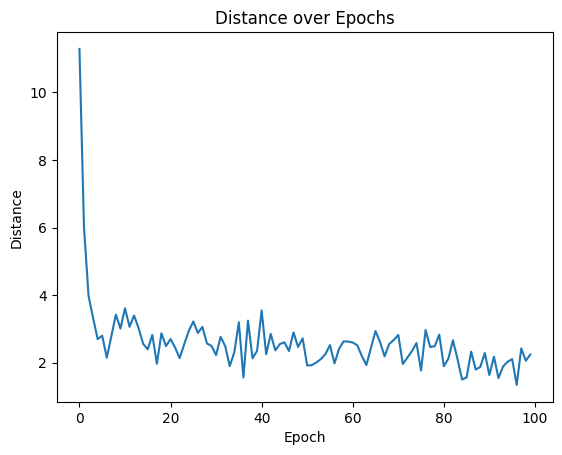
\includegraphics[width=0.8\textwidth]{Background/images/mean_std_cgan.png}
    \caption{Distance between real and generated parameters of the distribution over epochs.}
    \label{mean_std_distance}
\end{figure}


\begin{figure}[H]
    \centering
    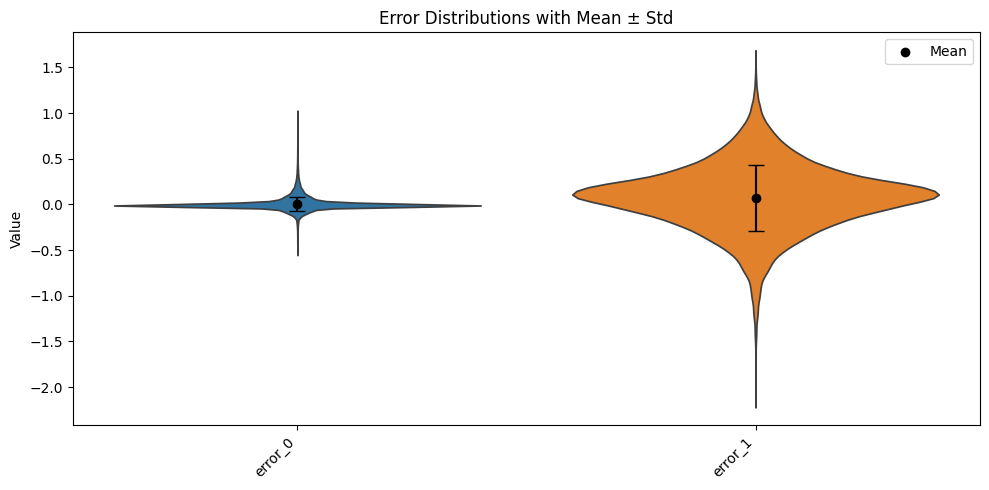
\includegraphics[width=0.9\textwidth]{Background/images/error_mean_std.png}
    \caption{Error distribution between real and generated parameters.}
    \label{mean_std_error}
\end{figure}




\section{Bins probabilities as target}
When the output representation is the bins probabilities of the normal distribution,
then logarithm transformation of the output data matrix $X$ is needed in order to avoid numerical issues and have a more stable training process.\\
In this case the distance between the real and generated distribution is measured by the Jensen-Shannon divergence
between the real and generated bins probabilities vectors.\\
However, instead of using just the Mean Absolute Percentage Error (MAPE) to run the error analysis between real and generated bins probabilities,
the Symmetric Mean Absolute Percentage Error (SMAPE) is used in order to take into account all those cases where
the real bin probability is equal to zero and that would lead to an infinite percentage error.


\subsection{Conditional GAN results}

On the first hand, a sketch of the algorithm and data flow used for training the CGAN model is shown below.
Then results obtained from training the CGAN architecture on the simulated dataset are presented.\\

\begin{algorithm}[H]
    \caption{Training process for CGAN model}
    \label{alg:cgan train}
    \begin{algorithmic}[1]

    \STATE Compute trajectories matrix $C$ and output data matrix $X$ using algorithm \ref{alg:y condition} and \ref{alg:x target}.
    \STATE Apply log transformation to data matrix $X$.
    \FOR{$i$ in $max\_epoch = 200$}
        \STATE Compute discriminator loss over true data samples $\mathcal{L}_{\text{BCE}}^{true}(1,D(x,c))
            = - \left[ 1 \log(D(x,c))\right]$ and then over generated data samples
            $\mathcal{L}_{\text{BCE}}^{fake}(0,D(G(z,c),c)) = - \left[  1\log(1 - D(G(z,c),c)) \right]$
        \STATE The Discriminator loss is then computed as $\mathcal{L}_D = \mathcal{L}_{\text{BCE}}^{true} + \mathcal{L}_{\text{BCE}}^{fake}$
        \STATE Update discriminator weights by backpropagating the loss $\mathcal{L}_D$.
        \STATE Compute generator loss over generated data samples
            $\mathcal{L}_{\text{BCE}}^{gen}(1,D(G(z,c),c)) = - \left[ 1 \log(D(G(z,c),c))\right]$   
        \STATE Update generator weights by backpropagating the loss $\mathcal{L}_G = \mathcal{L}_{\text{BCE}}^{gen}$.
    \ENDFOR
    \end{algorithmic}
\end{algorithm}

The experimental results have been obtained by training the CGAN model for 200 epochs, using the dataset and evaluation metrics described above with 
the following architecture and hyperparameters:
\begin{table}[h!]
\centering
\caption{CGAN Architecture and Hyperparameters Summary}
\label{tab:cgan_summary}
\begin{tabular}{lll}
\hline
\textbf{Parameter}         & \textbf{Generator}          & \textbf{Discriminator} \\ \hline
Input Dimension            & 252 (Latent) + 252 (Cond.)  & 100 (Data) + 252 (Cond.)         \\
Hidden Layers              & [512, 256, 256, 128]        & [512, 256, 256, 128, 64]        \\
Output Dimension           & 100                         & 1                               \\
Activation Function        & ReLU                        & Leaky ReLU                      \\
Normalization              & Batch Norm                  & None                      \\
Dropout                    & 0.0                         & 0.0                             \\
\multicolumn{3}{c}{\textbf{Global Training Settings}}                                     \\ \hline                                       \\
Generated Data Dimension (n of bins)             & \multicolumn{2}{l}{100}                             \\ \hline
Max Epochs                           & \multicolumn{2}{l}{200}                             \\ \hline
\end{tabular}
\end{table}


\begin{figure}[H]
    \centering
    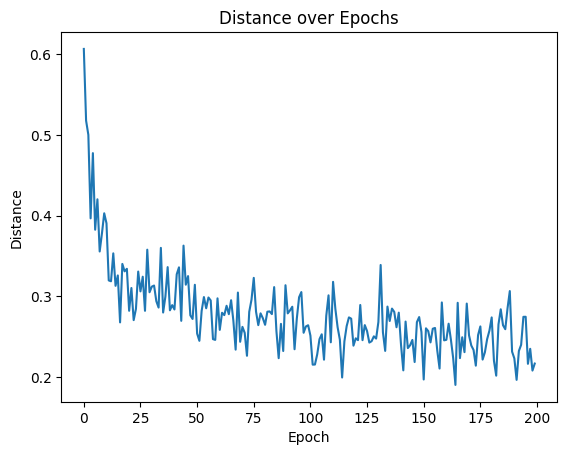
\includegraphics[width=0.9\textwidth]{Background/images/bins_global_distribution_cgan.png}
    \caption{Distance between real and generated probability density function using global bins.}
    \label{bins_global_distance}
\end{figure}

\begin{figure}[H]
    \centering
    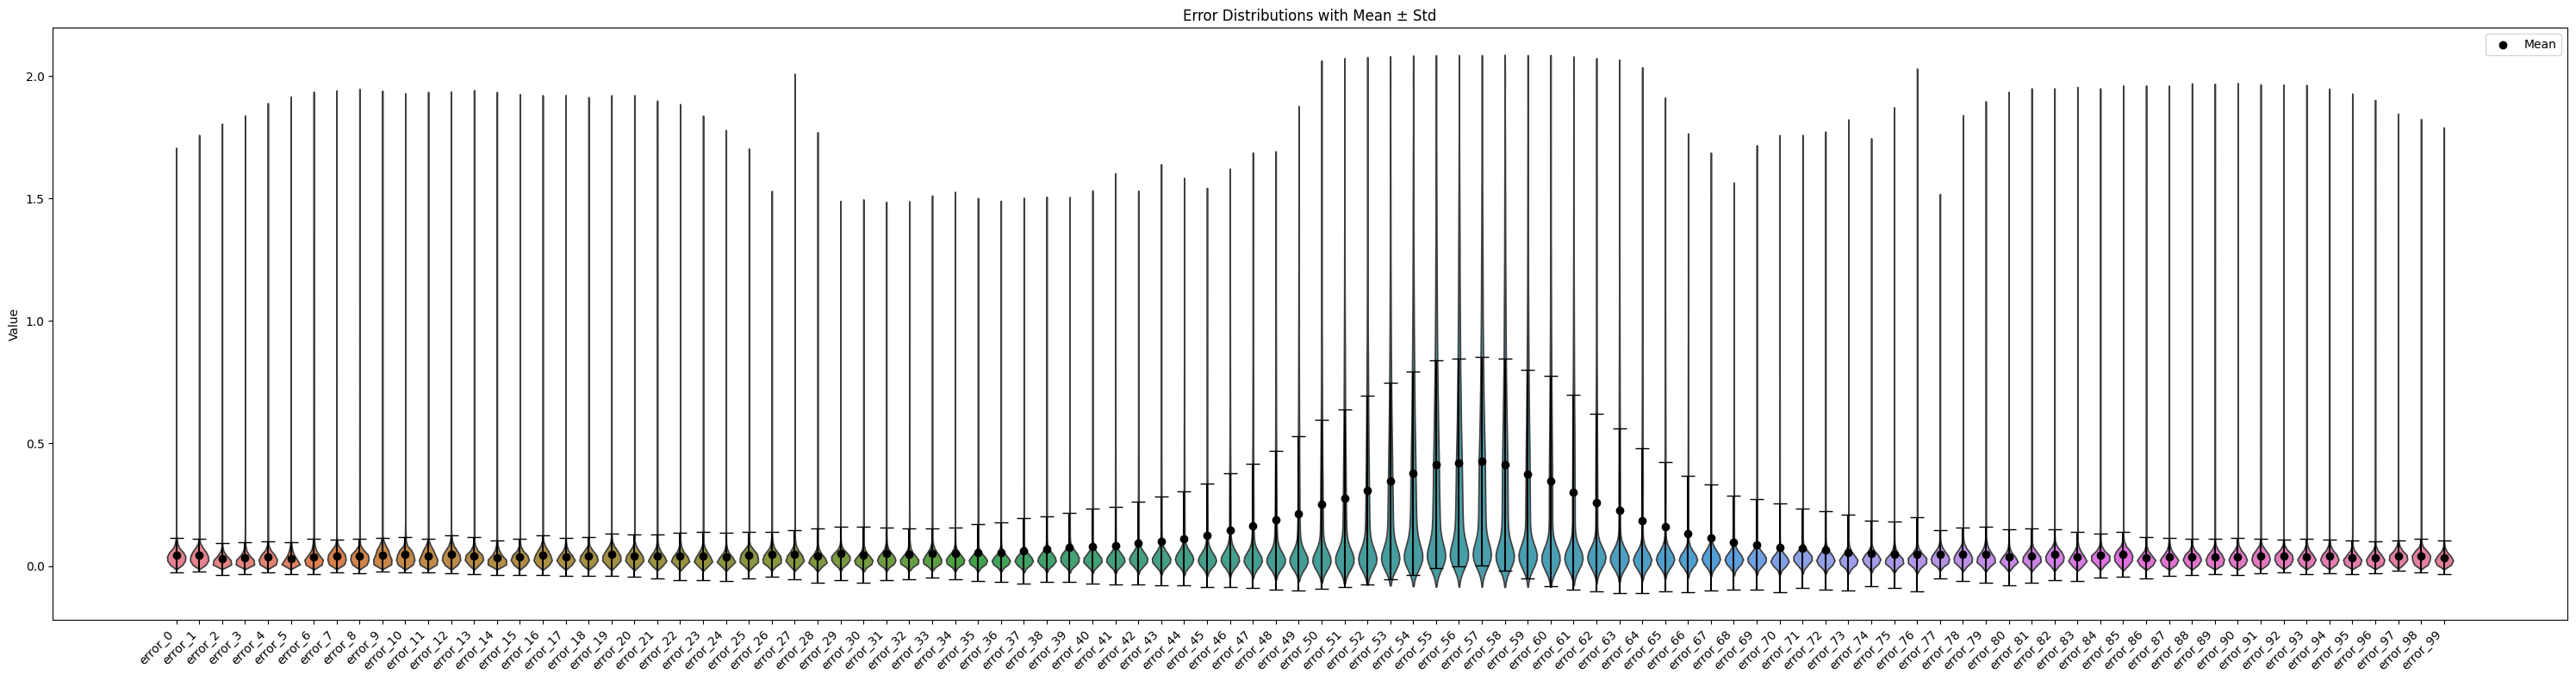
\includegraphics[width=0.9\textwidth]{Background/images/error_bins_global.png}
    \caption{Error distribution between real and generated bins probabilities using global bins.}
    \label{bins_global_error}
\end{figure}

From the results shown above in Figure \ref{bins_global_error}, it is possible to notice that tail bins have small error values since both real and generated probabilities tends to be close to zero.
Most of the errors are concentrated in central bins where the probabilities are higher and tends to be more variable. It is also important to notice the presence of error spikes,
suggesting that for some pairs of theoretical and generated distributions huge differences are present.\\
Also in this case the Kolmogorov-Smirnov test has been performed between 10000 real and generated bins probabilities, and
the resulting p-values are rejected 65\% of times, meaning that we can reject the null hypothesis
that the generated distribution are equivalent to the theoretical ones in 65 percent of the cases.\\

\begin{table}[h]
\centering
\begin{tabular}{l c}
\hline
\textbf{Metric} & \textbf{Value} \\
\hline
KS-Test acceptance rate & 0.35 \\
JS Distance & 0.3430 \\
Hellinger Distance & 0.3067 \\
TV Distance & 0.3078 \\
\hline
\end{tabular}
\caption{CGAN performance metrics averaged over 10000 samples}
\end{table}


In order to test the generalization capabilities of the model,
different samples have been drawn such that every sampling parameter is fixed except for the volatility $\sigma$.
In particular, six different samples are shown below where
the starting values is the same $X_0 = 0.0$, $\mu = 0.0$ while the volatility have different values for each sample 
$\sigma = [0.1, 0.3, 0.5, 0.7, 0.9, 0.11]$. 
\begin{figure}[H]
    \centering
    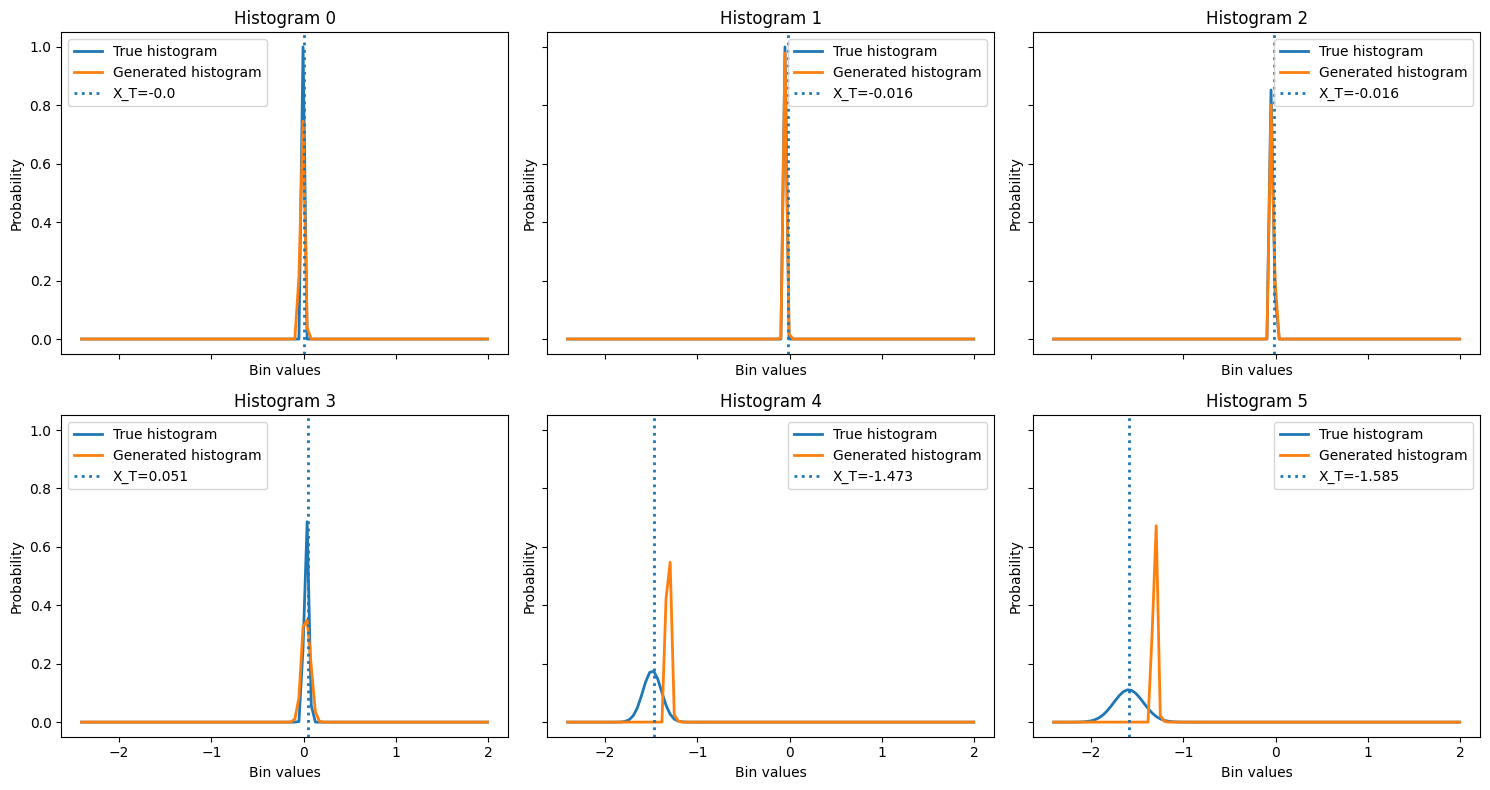
\includegraphics[width=1.0\textwidth]{Background/images/bins_samples_sigma.png}
    \caption{Samples obtained using fixed $X_0$ and $\mu$ while varying $\sigma = [0.1, 0.3, 0.5, 0.7, 0.9, 0.11]$.}
    \label{bins_global_sample_sigma}
\end{figure}

From the results shown above, it is possible to observe that the model is able to
effectively capture the first moment of the distribution since it is usually alligned with the theoretical distribution.
However, it struggles to accurately model the second moment, especially when the volatility is high.
This would lead to underestimate or overestimate tail risk in financial applications.

\subsection{Conditional Wasserstein GAN results}
In this section, we present the results obtained from training the CWGAN architecture on the same dataset used for the CGAN experiments, 
by following the same data simulation, preprocessing, and evaluation procedures described before.\\


\begin{algorithm}[H]
    \caption{Training process for CWGAN-GP model}
    \label{alg:cwgan train}
    \begin{algorithmic}[1]

    \STATE Compute trajectories matrix $C$ and output data matrix $X$ using algorithm \ref{alg:y condition} and \ref{alg:x target}.
    \STATE Apply log transformation to data matrix $X$.
    \FOR{$i$ in $max\_epoch = 100$}
        \STATE Compute the critic real value output for true data samples $D(x,c)$ and then for generated data samples $D(G(z,c),c)$.
        \STATE Compute the gradient penalty term $GP$ as defined in \ref{alg:gradient_penalty}.
        \STATE Compute critic loss $\mathcal{L}_D$ following \ref{alg:cwgan_gp} with the addition of the gradient penalty term.
        \STATE Update critic weights by backpropagating the loss $\mathcal{L}_D$.
        \STATE Compute generator loss $\mathcal{L}_G$ following \ref{alg:cwgan_gp}.
        \STATE Update generator weights by backpropagating the loss $\mathcal{L}_G$.
    \ENDFOR
    \end{algorithmic}
\end{algorithm}

The experimental results have been obtained by training the CWGAN-GP model for 100 epochs, using the same dataset and evaluation metrics as in the CGAN case with 
the following architecture and hyperparameters:
\begin{table}[h!]
\centering
\caption{CWGAN Architecture and Hyperparameters Summary}
\label{tab:cwgan_summary}
\begin{tabular}{lll}
\hline
\textbf{Parameter}         & \textbf{Generator}          & \textbf{Critic (Discriminator)} \\ \hline
Input Dimension            & 252 (Latent) + 252 (Cond.)  & 100 (Data) + 252 (Cond.)         \\
Hidden Layers              & [512, 256, 256, 128]        & [512, 256, 256, 128, 64]        \\
Output Dimension           & 100                         & 1                               \\
Activation Function        & ReLU                        & Leaky ReLU                      \\
Normalization              & None                        & Layer Norm                      \\
Dropout                    & 0.0                         & 0.0                             \\
\multicolumn{3}{c}{\textbf{Global Training Settings}}                                     \\ \hline                                       \\
Generated Data Dimension (n of bins)           & \multicolumn{2}{l}{100}                          \\ \hline   
Max Epochs                           & \multicolumn{2}{l}{100}                                       \\ \hline
\end{tabular}
\end{table}

\begin{figure}[H]
    \centering
    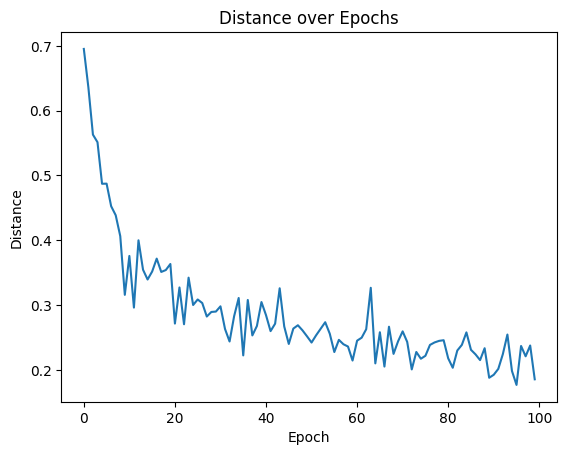
\includegraphics[width=0.9\textwidth]{Background/images/bins_global_distribution_cwgan.png}
    \caption{Distance between real and generated probability density function of the standard normal distribution over epochs.}
    \label{cwgan_curve}
\end{figure}



\begin{figure}[H]
    \centering
    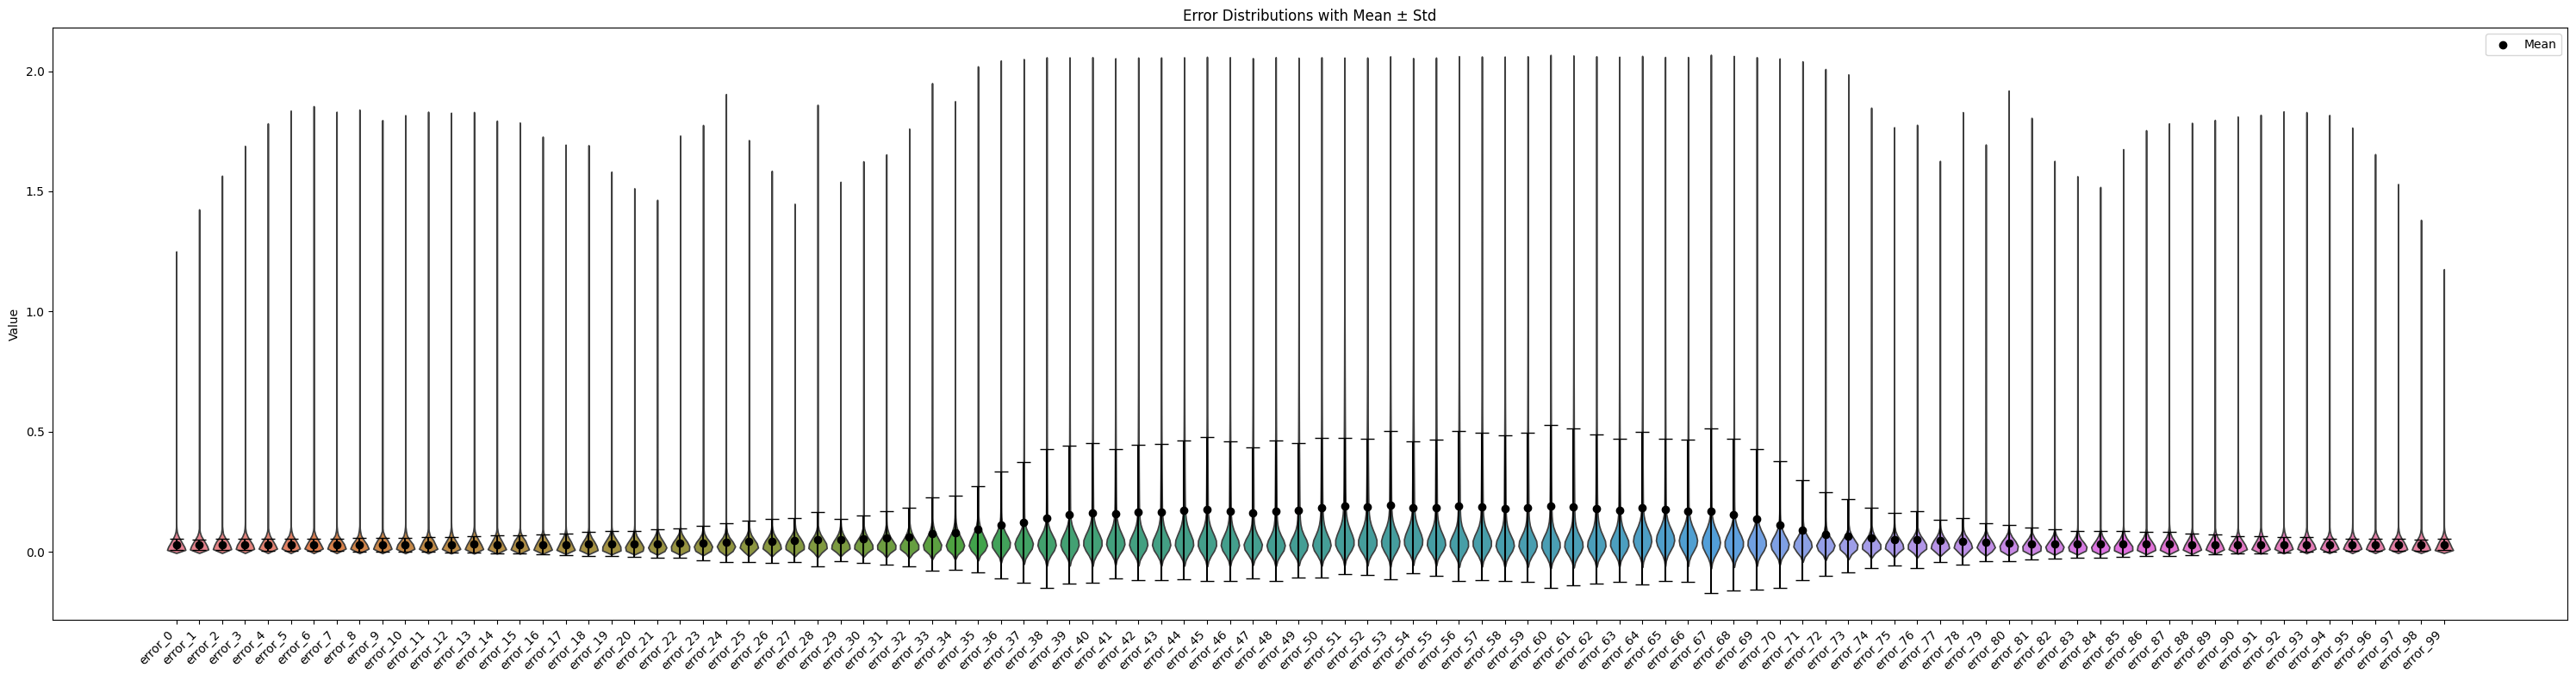
\includegraphics[width=1.0\textwidth]{Background/images/CWGAN_error_dist.png}
    \caption{Error distribution between real and generated bins probabilities using global bins.}
    \label{cwgan_global_error}
\end{figure}



\begin{figure}[H]
    \centering
    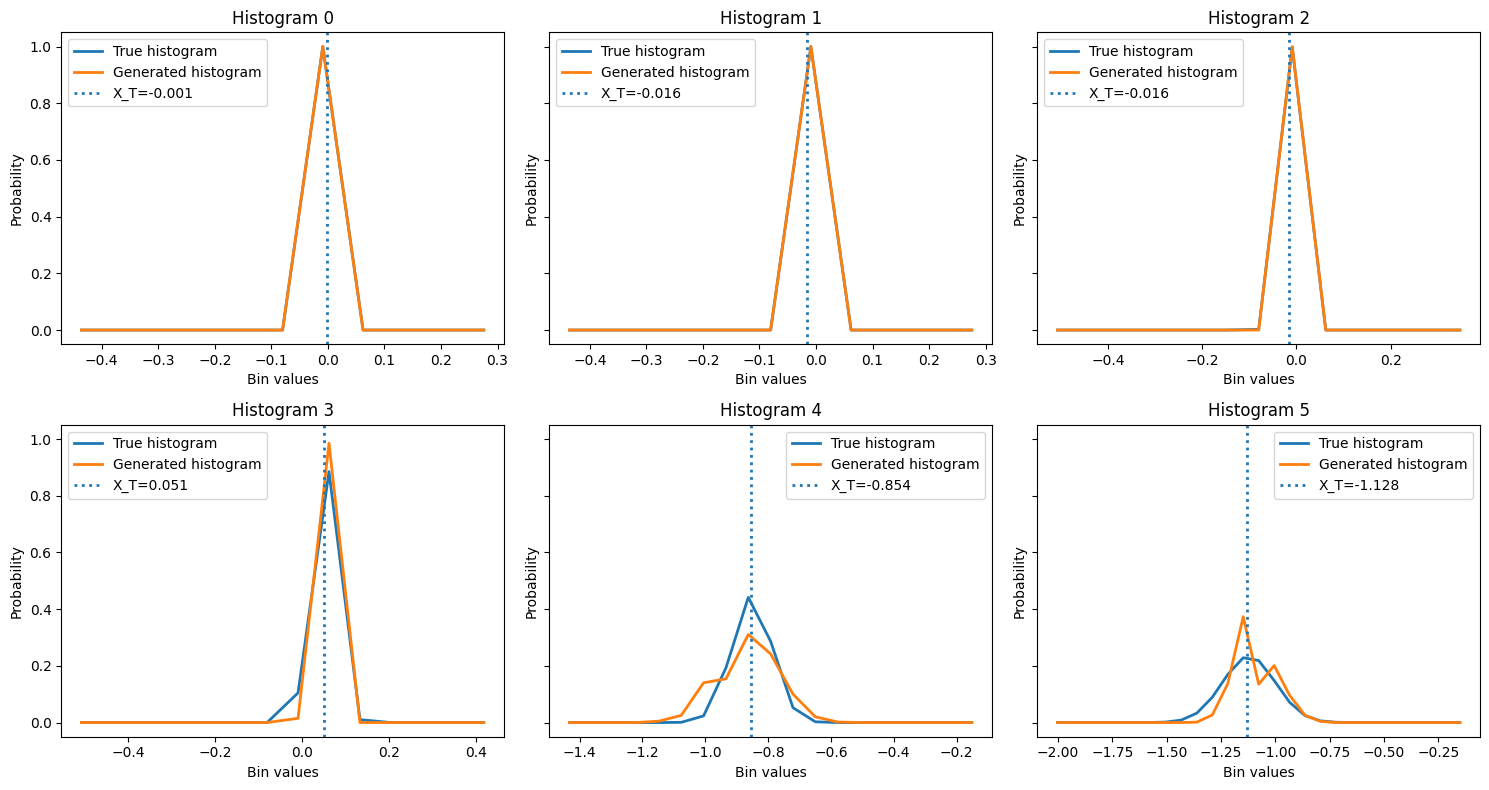
\includegraphics[width=1.0\textwidth]{Background/images/cwgan_samples_sigma.png}
    \caption{Samples obtained using fixed $X_0$ and $\mu$ while varying $\sigma = [0.1, 0.3, 0.5, 0.7, 0.9, 0.11]$.}
    \label{cwgan_sample_sigma}
\end{figure}


As can be seen from \ref{cwgan_sample_sigma} the quality of the generated distributions is significantly improved with respect to the CGAN results shown in \ref{bins_global_sample_sigma}.
This is also confirmed by running the Kolmogorov-Smirnov test over 10000 generated samples. The results show that
53\% of the generated samples are accepted at a significance level of 1\%, compared to only 35\% acceptance rate for the CGAN model.\\

\begin{table}[h]
\centering
\begin{tabular}{l c}
\hline
\textbf{Metric} & \textbf{Value} \\
\hline
KS-Test acceptance rate & 0.53 \\
JS Distance & 0.3050 \\
Hellinger Distance & 0.2712 \\
TV Distance & 0.2725 \\
\hline
\end{tabular}
\caption{CWGAN-GP performance metrics averaged over 10000 samples}
\end{table}

However, the model still provide poor performances since for higher values of $\sigma$ the generated distributions tends to be rejected from the KS test, suggesting lack of capacity to model the full range of the target distribution for trajectories with high volatility.
Moreover, the average Jenshen-Shannon divergence between real and generated distributions over the 10000 samples is around 0.20 which is not an excellent result considering that the JS-divergence is bounded between 0 and 1.
These poor performances arises from the main drawback of the proposed architecture, which is the discretization of the output distribution into a fixed number of bins. 
This approach can lead to loss of information and may not capture the full complexity of the underlying distribution, especially in cases where the chosen number of bins is insufficient to represent the true distribution, particularly if the distribution has heavy tails or is multimodal.

\section{Possible improvements}
The main issue that need to be addressed in order to produce coherent distributions is to produce a meaningful representation of the output to be generated 
in order to effectively capture the variance of the target distribution, 
avoiding in this way underestimation or overestimation of extreme events.
Different approaches have been adopted in the literature to adapt the GAN architecture to time series data, with the aim
of improving training stability, convergence of GANs and solve the mode collapse problem.\\

Specific techniques can be employed to better capture the distributional characteristics of financial time series data.
Some of these techniques are discussed in academic papers like \cite{background:forgan}, \cite{background:md_cgan} and \cite{background:rcgan}:
\begin{itemize}
    \item For example, in \cite{background:rcgan} both the generator and discriminator are RNN or LSTM networks adopted to better capture the sequential dependencies in time series data.
    \item Predict the values corresponding to a fixed set of quantiles. 
    The model generates the outcome values associated with specified probability levels for example $[0.01, 0.1, 0.25, 0.5, 0.75, 0.9, 0.99]$.
    Usually this approach is used in quantile regression where the loss function is the quantile loss, which is specifically designed to provide consistent estimation of conditional quantiles.
    \item Model the output distribution as a mixture of Gaussians, where the generator predicts the parameters of the mixture components (means, variances, and mixing coefficients) as proposed in \cite{background:md_cgan}.
    \item The generated output can be the value of the time step for which we would like to generate the distribution. So after training,
    at inference time, the distribution can be recovered by repeatedly evaluating the generator for a fixed input trajectory while varying the random noise.
    The collection of generated outputs, for example 1000 samples, constitutes an empirical approximation of the conditional predictive distribution as discussed in \cite{background:forgan}.
    \item Adding a term to the generator's loss that penalizes it if the mean and variance of a batch of generated samples don't match the mean and variance of the "real" theoretical samples.
\end{itemize}

However, in this work, the focus is on the architecture proposed in \cite{background:forgan} possibly with some improvements in order to generate a more meaningful representation of the output distribution, for 
financial processes characterized by high volatility and heavy tails. The proposed architecture is discussed in the next chapter.
